\section{研究背景}
Spiking Neural Network (SNN)は, 通常のArtificial Neural Network (ANN)と比較して, より脳神経回路を模した数理モデルである.
脳における電気パルス信号を介した神経ダイナミクスを数理モデルとして持つため, SNNはその生物学的妥当性が高い\cite{taherkhani2020review}.
また, SNNはニューロモーフィックデバイスと呼ばれる専用の計算機を用いて実装することでその消費電力を削減できることも知られている\cite{balaji2019mapping}.
その適用範囲は広く, 物体認識 (\tabref{tab:snnyolo}) や言語モデル (\tabref{tab:spinnaker}) , ロボットの自己位置推定とマッピング (\figref{fig:snnslam}) などのタスクにおいてその有効性が示されている\cite{yamazaki2022spiking, snnyolo, s23063037, spinnaker,snnslam}.
さらに, SNNは入力ノイズに対する頑健性が高いとされている.
ガウシアンノイズなどの画像認識における入力画像へのノイズに対する頑健性 (\figref{fig:robust:gaussian}) \cite{zhao2022spiking}や, SNNを用いて学習した強化学習エージェントのノイズによるパフォーマンス低下を抑制する結果 (\figref{fig:robust:atari}) が報告されている\cite{patel2019improved}.
このような特性から, SNNは次世代のニューラルネットワークとしての関心を集めている\cite{maass1997networks, wang2020supervised}.

一般に, 時系列信号は信号速度の変化や多量の周波数情報を持つが, 生物の脳はそのような信号に対して頑健な処理を行うことが可能である.
% 例えば, 異なる速度で話す話者であっても, 人は容易に内容を認識することができるなどが挙げられる.
例えば, 音声認識や動画認識において, 内容が同じであれば, 人はその速度に依らずに同一の認識を行うことが可能である.
これは, 脳が領域によって異なる時間的特性を持ち, その学習を行うからであると考えられている\cite{mattia2002population, deco2019brain}.
したがって, 脳神経回路を模したSNNにおいても, 時系列信号に対する表現力の高さと頑健性が期待される\cite{dhsnn}.

しかしながら, 既存のSNNのほとんどはこのような時間的特性を十分に活用できていない\cite{dhsnn}.
SNNにおける神経細胞ダイナミクスのモデル化には, 数理的な扱いやすさと計算コストの低さからLeaky Integrate-and-Fire (LIF)モデルが多く採用されている.
LIFモデルは, それぞれの神経細胞への入力である電気パルス信号とその神経細胞の膜電位の関係を微分方程式によってモデル化したものである.
% ここで, 膜電位はその神経細胞への過去の入力信号が反映された情報であり, 膜電位の値に従って, 接続された別の神経細胞への入力信号が決定される.
% このような過去の情報の記憶にあたる膜電位は時間経過によって減衰する.
ここで, 膜電位は入力情報の時間的な蓄積を表すものである.
SNNが学習されるに従って, 膜電位は重要な時間関係が現れた際に活性化されるようになる.
さらに, 膜電位が活性化されたニューロンは次のニューロンへ信号が伝達するように振る舞う.
このように, 膜電位が時間関係の表現に重要な役割を果たすことで, SNNが時間的なタスクを学習することが可能となる.
LIFモデルでは, 膜電位は情報の入力と時間経過による減衰によって値が決定される.
この減衰量を決定するパラメータとしてLIFモデルは時定数を持つが, モデルの設計者が扱う問題に応じて設定し, その後更新されることはない.
また, 時定数はSNNにおける全てのニューロンで同じ値を適用する.
このような時定数の学習不可能性と単一性は, 脳の異なる領域における多様な時間的特性とその学習能力と乖離しており, SNNの時系列信号に対する表現力と頑健性の向上の制限となる.


\begin{figure}[htb]
    \centering

    \begin{minipage}{0.3\textwidth}
        \centering
        \includesvg[width=0.8\textwidth, inkscapelatex=false]{Static/chap1_lowpower_slam}
        \subcaption{SLAM using SNN\cite{snnslam}}
        \label{fig:snnslam}
    \end{minipage}
    \hspace{0.02\textwidth}
    \begin{minipage}{0.6\textwidth}
        \centering
        \begin{tabular}{ccc}
            \hline
            & Nvidia A100 & SpiNNaker2 \\ 
            \hline
            Power (W) & 60 & \textbf{0.39} \\
            Energy (J) & 1.1935 & \textbf{0.0653} \\
            Test PPL & 79.3 & 79.3 \\
            \hline
        \end{tabular}
        \subcaption{SpiNNaker2\cite{spinnaker}}
        \label{tab:spinnaker}
    \end{minipage}


    \begin{minipage}{1.0\textwidth}
        \centering
        \begin{tabular}{cccccc}
            \hline
            \multicolumn{6}{c}{\textbf{Tiny YOLO}}\\
            \hline
            &Power (W) & GFLOPS & FLOPs & & Energy (J) \\
            &250 & 14,000 & 6.97E+09 & & 0.12 \\
            \hline
            \multicolumn{6}{c}{\textbf{Spiking-YOLO}}\\
            \hline
            method & GFLOPS / W & FLOPs & Power (W) & Time steps & Energy (J) \\
            method1 & 400 & 5.28E+07 & 1.320E-04 & 8,000 & \textbf{1.06E-03} \\
            method2 & 400 & 4.90E+07 & 1.225E-04 & 3,500 & \textbf{4.29E-04} \\
            \hline
        \end{tabular}
        \subcaption{Spiking YOLO\cite{snnyolo}}
        \label{tab:snnyolo}
    \end{minipage}

    \caption[SNNの低消費電力性能]{
        SNNの低消費電力性能.
        (a) SLAMによるロボットの自己位置推定とマッピングにおける消費電力. 
        CPUと比較して, SNNで実装したLoihiの消費電力が小さい.
        (b) ニューロモーフィックデバイスSpiNNaker2で実装した単語推定における消費電力. 
        (c) SNNを用いた物体認識における消費電力. 従来のTiny YOLOと比較して, SNNを用いたSpiking-YOLOは消費電力が小さい.
    }
\end{figure}


\begin{figure}[htb]
    \centering

    \begin{minipage}{0.45\textwidth}
        \centering
        \includesvg[width=1.0\textwidth, inkscapelatex=false]{Static/chap1_robust_gaussian}
        \subcaption{Gaussian noise\cite{zhao2022spiking}}
        \label{fig:robust:gaussian}
    \end{minipage}
    \hspace{0.02\textwidth}
    \begin{minipage}{0.45\textwidth}
        \centering
        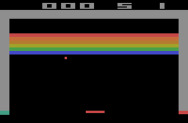
\includegraphics[width=1.0\textwidth]{Static/chap1_robust_atari.jpg}
        \subcaption{Atari game scene\cite{patel2019improved}}
        \label{fig:robust:atari}
    \end{minipage}

    \caption[SNNの頑健性]{
        SNNのノイズに対する頑健性.
        (a) ガウシアンノイズに対するSNNの頑健性. 
        SNNを用いた識別モデルはノイズ強度の増加による性能の劣化が小さい.
        (b) Atariゲームにおけるブロック崩し.
        SNNを用いた強化学習エージェントは, 画面の一部を隠した際のスコア低下が小さい.
    }
\end{figure}

